\chapter{Introduction}
% Text goes here
\subsection{What happened and how it began}
Over the past decades, the video game industry has experienced substantial and sustained growth, becoming one of the most relevant sectors within the global digital economy and surpassing several traditional entertainment industries in terms of revenues (\cite{npd2009more}).
\\\\
This industry emerged in the 1970s as a niche form of entertainment and it
gradually expanded through the development of home consoles and personal computer gaming. The introduction of platforms such as the Nintendo Entertainment System (NES) in the 1980s contributed to the diffusion of video games into households, revitalizing the video game industry in the US and marking the beginning of the home gaming era \cite{ebsco_nes}.
\\\\
A further structural transformation occurred in the late-1980s with the emergence of advanced console generations and the commercialization of video games as mainstream entertainment products. In this period, with the introduction of the World Wide Web by the scientist Tim Berners-Lee -- whose objective was to merge the evolving technologies of computers and data networks into a powerful and easy to use global information system --, the industry experienced a shift towards digitalization, characterized by online gaming, downloadable content (DLC), and continuous post-purchase updates, allowing small creators to challenge big companies with free or inexpensive games \cite{WWW_Birth, ebsco_rise_video_games, dlcs}. 
\\\\
This transition marked the beginning of a new business model in which revenues were increasingly driven not only by initial sales but also by ongoing digital services and network-based consumption.

\subsection{Why did it grow}
Technological progress represents one of the principal drivers of growth in the video game industry. Early video games were characterized by extremely simple graphics and limited computational capabilities (like the first video game "Tennis For Two" developed in 1978). 
\begin{figure} [H]
    \centering
    
\includegraphics[width=0.5\linewidth]{img/Tennis_For_Two.jpg}
    \caption{Tennis For Two}
    \label{fig:Tennis}
\end{figure}

However, continuous advancements in hardware and software have significantly enhanced the quality and complexity of gaming experiences.
\\
The introduction of dedicated graphics processing units (GPUs) enabled the development of three-dimensional environments and more realistic rendering, increasing so the attractiveness of video games to a broader audience. Furthermore, as said before, the emergence of online gaming marked a fundamental shift in the industry, allowing users to interact in real time and creating network effects that contributed to the expansion of the user base \cite{esa2024, nvidia_raytracing,intel_gpu}.\\
More recent innovations, such as cloud gaming and artificial intelligence, have further reduced entry barriers and improved user engagement. Cloud gaming, in particular, allows users to access high-quality games without the need for advanced hardware, while AI technologies enhance gameplay through adaptive environments and personalized experiences \cite{redbull_ai_gaming, xbox_cloud_gaming}.\\
Overall, these technological advancements have not only improved product quality but have also contributed to the expansion of the market and the increase in industry revenues.


\subsubsection{Mobile Gaming}
Mobile gaming represents one of the most significant drivers of expansion in the video game industry over the past decade. The widespread diffusion of smartphones has substantially lowered entry barriers, allowing a much broader segment of the population to access video games.
\\
According to \cite{esa2024}, a large proportion of gamers engage with video games through mobile devices, with usage rates reaching approximately 78.8\% across different age groups in the United States. This highlights the role of mobile platforms in expanding the user base beyond traditional console and PC gamers.
\\
From an economic perspective, mobile gaming has contributed to industry growth by increasing market size and enabling new forms of monetization, particularly through free-to-play models and in-app purchases.
\\\\

\subsubsection{New Business Models}
Another key factor behind the growth of the video game industry is the evolution of business models, which has significantly transformed the way revenues are generated. Traditionally, video games were primarily distributed through a pay-to-play model, where users purchased a game once and retained full access. \\
However, the industry has progressively shifted towards more flexible and diversified monetization strategies. The emergence of freemium models, for example, allows users to access games for free while generating revenues through in-game purchases, such as cosmetic items or gameplay enhancements. This approach has proven particularly effective in expanding the user base while maintaining strong revenue streams (with most performative games generating a revenue per user comprehended in the interval between \$1-\$5 \cite{freemium_game_models}). \\
Additionally, downloadable content (DLC) and expansion models have enabled firms to extend the lifecycle of games, generating continuous revenues beyond the initial sale. Subscription-based services, such as platform-specific gaming passes, have further reinforced recurring revenue streams by offering access to large libraries of games for a fixed periodic fee \cite{xbox_game_pass} \cite{playstation_plus}. \\
Other monetization strategies include advertising-based models, particularly common in mobile gaming, and loot box systems, which introduce randomized rewards and have been widely discussed in the literature due to their similarities to gambling mechanisms \cite{LootBox_Model}.\\
\\\\

\subsubsection{Social Effect}
Social dynamics represent another driver of growth --that is worth to mention-- in the video game industry, particularly through the presence of network effects. The value of many video games, in fact, increases as the number of users expands, especially in multiplayer and online environments.
\\
In this context, digital platforms such as Twitch and YouTube have played a crucial role in amplifying the visibility of video games, allowing content creators to reach large audiences and influence consumer behavior. This form of indirect promotion has contributed to the rapid diffusion of games across different segments of the population.\\
In fact, according to statistics, more than 40\% of players discover new games through streams, giving even small studios a chance to rise in the charts without huge budgets if their game is noticed and shown by a popular content creator \cite{streaming_game_popularity} \cite{impact_game_streaming_industry}. \\
For many viewers it is more interesting to watch the stream than to run the game alone. Thus, the popularity of the game can be measured not only by the number of active players, but also by the number of hours of viewing \cite{streaming_game_popularity} .
\\
From an economic perspective, these mechanisms reinforce demand by creating positive feedback loops, where increased visibility leads to higher adoption rates, which in turn enhances the attractiveness of the product.

 

\subsubsection{The core reason because people play video games}

Understanding the underlying motivations that drive individuals to engage with video games is essential to explain the sustained growth in demand. Video games provide a combination of entertainment, cognitive stimulation, and social interaction, making them an attractive form of leisure activity across different demographic groups.
\\
Empirical evidence supports this view. According to \cite{esa2024} \ref{fig:Why_People_Play_Videogames}, a large portion of players report that gaming contributes positively to their cognitive and social skills. For instance, 73\% of gamers believe that video games improve problem-solving abilities, while 64\% associate gaming with enhanced teamwork and collaboration skills.\\
These factors contribute to the persistence of demand over time, reinforcing the position of video games as a central component of modern digital entertainment.

 
\begin{figure} [H]
    \centering
    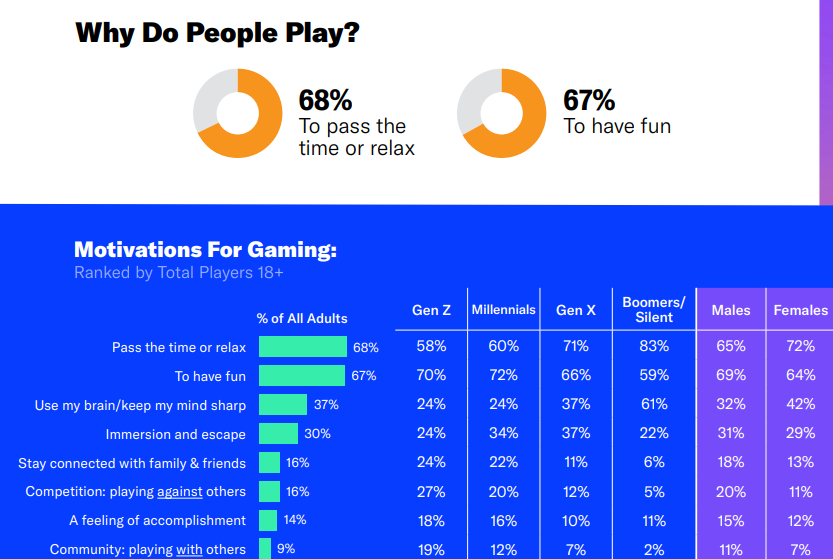
\includegraphics[width=0.5\linewidth]{img/Why_People_Play_Videogames.png}
    \caption{Why people play video games}
    \label{fig:Why_People_Play_Videogames}
\end{figure}




\subsection{The market}
The video game market has undergone significant structural changes over the past decades, characterized by a substantial expansion of its user base. The increasing diffusion of online gaming has played a central role in this transformation. According to \cite{esa2024}, the share of players engaging in online gaming in the United States increased from approximately 18\% in 1999 to nearly 90\% in recent years, highlighting the growing importance of connectivity in modern gaming experiences.\\
In addition, the demographic composition of the gaming population has become increasingly diversified. Contrary to the traditional perception of video games as a form of entertainment primarily targeted at younger audiences, recent data indicate that a large proportion of adults actively engage in gaming activities \ref{fig:Grafico_ESA}. This shift has contributed to a broader and more stable demand base.  
\begin{figure} [H]
    \centering
    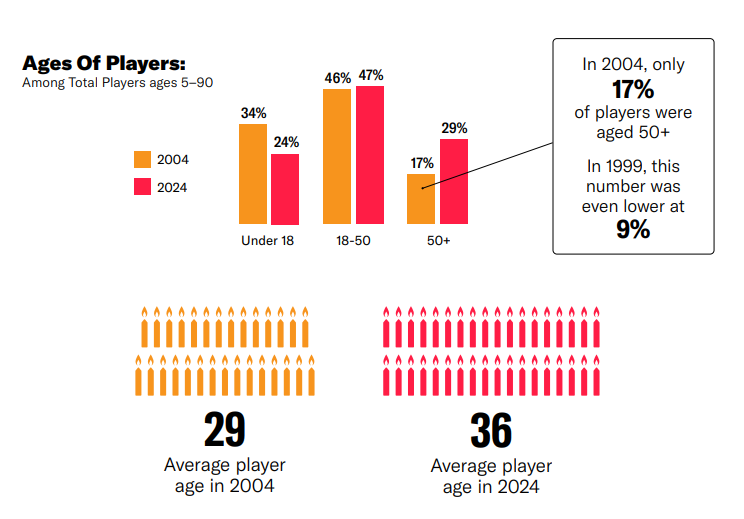
\includegraphics[width=0.5\linewidth]{img/Screenshot 2026-05-02 010839.png}
    \caption{Graph from ESA 2024}
    \label{fig:Grafico_ESA}
\end{figure}
Furthermore, gender distribution within the gaming population has become increasingly balanced, suggesting that video games have evolved into a mass-market form of entertainment rather than a niche activity. These structural changes in the user base have played a key role in supporting the long-term growth of industry revenues \ref{fig:Males and Females}. 

\begin{figure} [H]
    \centering
    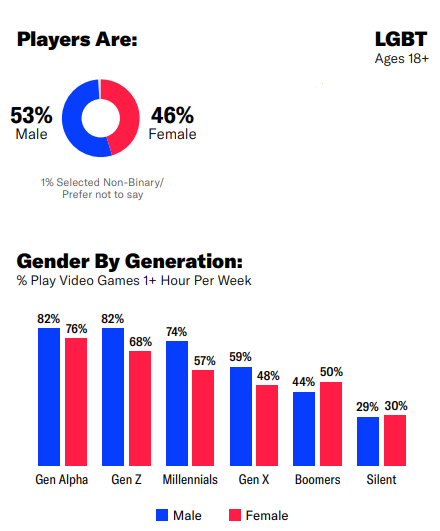
\includegraphics[width=0.5\linewidth]{img/Grafico_ESA_MF.png}
    \caption{Males and Females in Video games}
    \label{fig:Males and Females}
\end{figure}

\subsection{The purpose of this project}
While the video game industry has experienced strong structural growth over the past decades, understanding the drivers behind this expansion requires distinguishing between long-term economic and technological factors and short-term shocks such as the COVID-19 pandemic. The pandemic can be interpreted as a temporary demand shock that significantly accelerated industry revenues, followed by a period of normalization after 2021.

In this context, this study aims to analyze the evolution of video game industry revenues over the period 2014–2024, identifying the key macroeconomic and socio-demographic determinants of growth. In particular, the analysis focuses on variables such as income levels, inequality, population size, mental health indicators, and government restrictions during the pandemic period, in order to assess their impact on industry performance.

 